\chapter{Arbetet}
Arbetet kan del


Stort problem är att json och json scheman inte skiljer på heltal och reela tal, medan många språk gör det. Specifikt Delphi som systemet utvecklades i.

\section{Systemet i helhet}

När administrationsprogrammet kopplar upp sig mot servern skickar servern ett JSON Schema, tillsammans med en JSON-fil som beskriver den riktiga datan. Det flödet illustreras i figur \ref{fig:system:ner}. Hur datan sedan propageras upp från användargränssnittet, till servern illustreras i figur \ref{fig:system:upp}.

\begin{figure}
	\begin{subfigure}[b]{0.5\textwidth}
		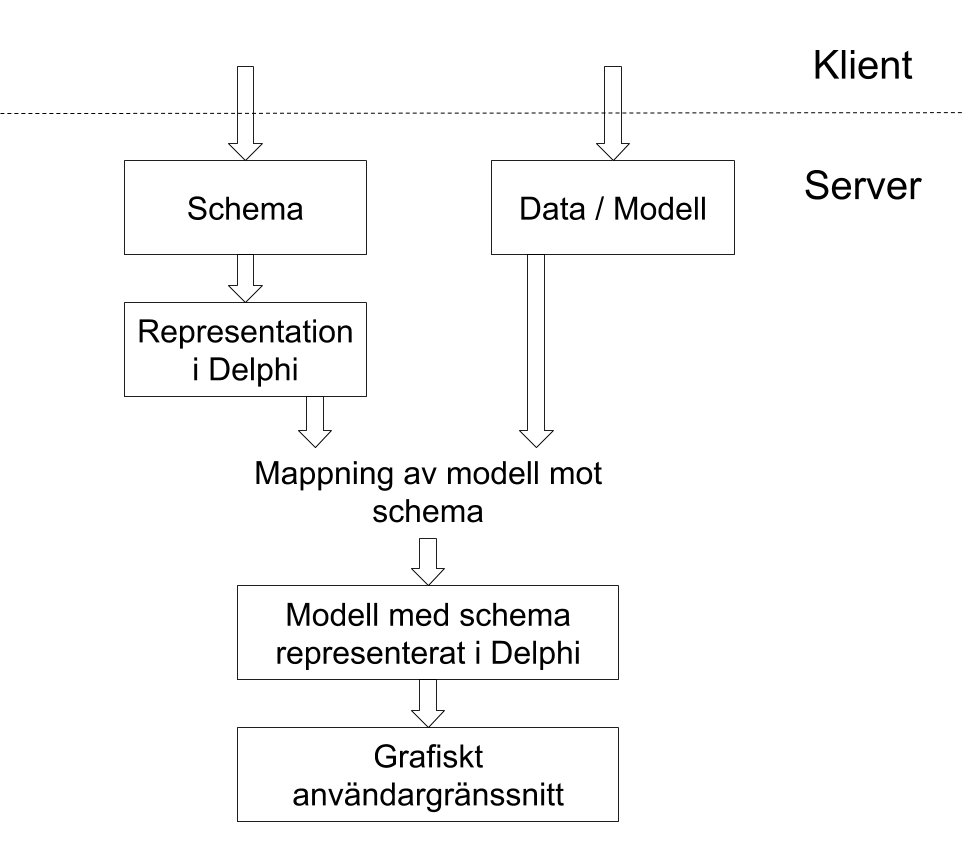
\includegraphics[width=0.9\textwidth,left]{./images/system-ner.png}
		\caption{Flödesschema över systemet}
		\label{fig:system:ner}
	\end{subfigure}
	\begin{subfigure}[b]{0.5\textwidth}
		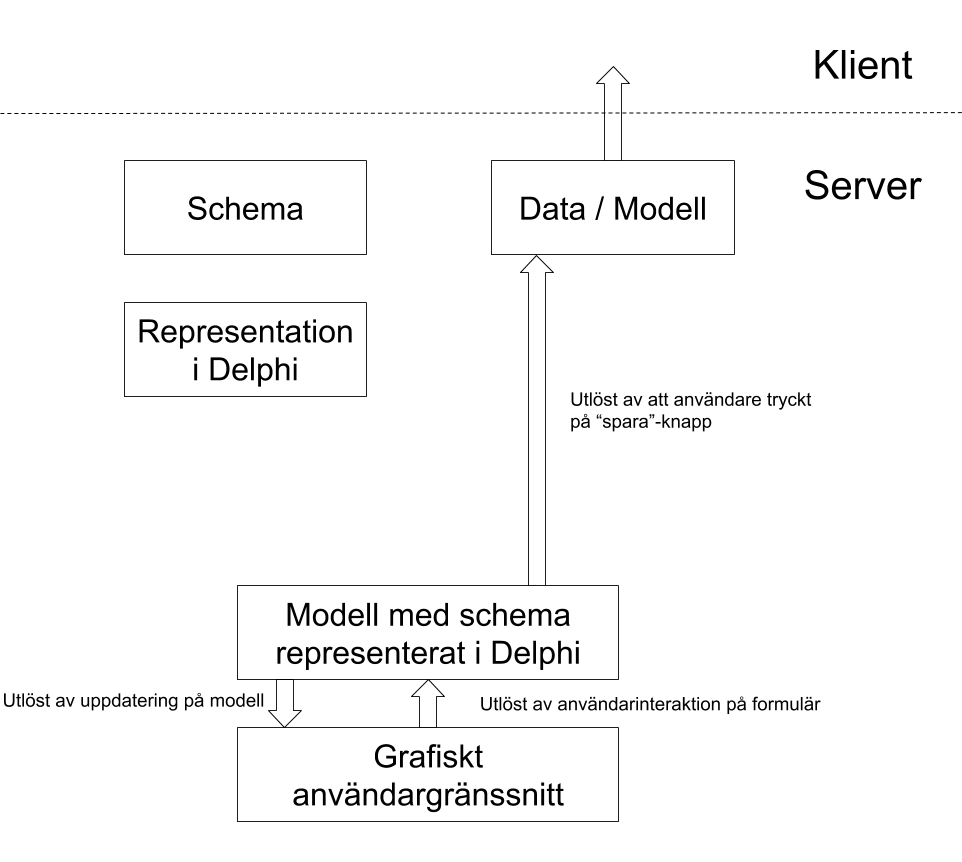
\includegraphics[width=0.9\textwidth,right]{./images/system-upp.png}
		\caption{Flödesschema över systemet}
		\label{fig:system:upp}	
	\end{subfigure}
	\caption{Illustration av dataflöde till och från användargränssnittet}
	\label{fig:system}
\end{figure}

\section{Generering av JSON Schema i Delphi}

Hur JSON Schemat genereras, påverkar inte slutanvändaren, men det påverkar utvecklarna som ska jobba med systemet, och kan hindra vilken funktionalitet som finns tillgänglig i systemet. Ett alternativ är självklart att skriva scheman för hand, men då olika klienter måste ha olika scheman, måste utvecklare se till att rätt schema hamnar på rätt klient vid instalationen av Mimer SoftRadio. Om en kund skulle vilja uppgradera funktionaliteten hos sin installation av Mimer SoftRadio, och därmed behöva tillgång till fler konfigurerbara inställningar i systemet, skulle schemat behöva uppdateras efteråt.

Ett annat alternativ är att basera schemat på inbyggda datatyper i det statiskt typade språket Delphi. Json.NET Schema, NJsonSchema for .NET, typescript-json-schema samt Typson erbjuder exakt den här funktionaliteten i språken .NET respektive TypeScript. För att lägga till extra beskrivningar av datan som språket inte räcker till för, använder .NET-implementationerna \textit{Data Annotation Attributes}, och TypeScript-implementationerna använder experimentella \textit{Decorators}. \cite{Suter,Newtonsoft,El-Dardiry,Bovet} Delphi erbjuder liknande funktionalitet med \textit{Attributes (RTTI)} \cite{Embarcadero2016}. Att annotera datastrukturerna som faktiskt sedan kommer användas i ett system kan automatisera väldigt mycket. Det passar jättebra om det handlar om att bygga ett API där JSON Scheman ska användas för att beskriva för klienter hur och vilken data de kan manipulera. Då kan scheman dynamiskt skapas vid exekvering och de är alltid synkroniserade med datan som systemet är konstruerat för att hantera. Problemet med den lösningen är att schemat i det här arbetet inte ska användas för att beskriva vilken data som kan manipuleras på servern, utan det ska användas för att beskriva hur ett användargränsnitt ska se ut. Den data som ska presenteras på användargränsnittet är en delmängd av all tillgänglig data på servern. Det skulle kunna gå att lägga till annoteringar som beskriver vilken data som ska finnas med på schemat, men det finns enklare lösningar.

Alternativet att handskriva JSON Scheman kräver mycket uppräthållning av scheman och är väldigt mottagligt för misstag hos utvecklarna. Det kräver dock inget system för att dynamiskt generera scheman vid exekvering, då de redan skulle vara genererade. Alternativet att konstruera ett system som använder run-time type information \textit{(RTTI)} är väldigt smidigt för utvecklare under exekvering men kräver relativt mycket utveckling. Ett mellanting skulle vara felsäkert som handskrivna JSON Scheman, men samtidigt dynamiskt genererat vid exekvering för felfria scheman.

JSL är ett exempel på en implementation som erbjuder specifika komplexa datatyper som underlättar genererandet av JSON Scheman. JSL skiljer på datastrukturerna som används för att representera och manipulera data, och själva schemat som används för att beskriva de tidigare nämnda datastrukturerna. \cite{Romanovich} Det ansågs vara ett väldigt praktiskt mellanting. Scheman skrivs för hand men de skrivs inte som JSON Scheman. Istället skrivs de som instanser av komplexa datatyper i Delphi, som sedan under exekvering dynamiskt tolkas för att generera ett JSON Schema. Det här tillåter servern att under exekvering utföra logiska bedömningar för att inkludera exakt det som ska inkluderas i schemat, beroende på vilken version av Mimer SoftRadio operatörsdatorn har, och med vilken tillgänglig funktionalitet datorn har. Schemagenerering är frikopplat från databehandling, men är samtidigt dynamiskt genererat utifrån tillgänglig funktionalitet på operatörsdatorn.

Att generera scheman från JSON-filer ansågs inte vara praktiskt genomförbart (se kapitel \ref{sec:forarbete:json-till-schema}), och skulle inte kunna uppräthålla kraven på systemet. Det skulle dessutom helt ta bort möjligheten för utvecklare att beskriva användargränssnittet.

\section{Parsningen av JSON Schema i Delphi}


\section{Representation av data i användargänssnittet}

\begin{figure}
	\inputminted[tabsize=2, frame=single, fontsize=\tiny, framesep=2mm, breaklines]{json}{code/schema.json}
	\vspace{-1.7em}
	\caption{Exempel på genererat schema}
	\label{fig:real-schema}
\end{figure}

\section{Manipulering av data utifrån användarinteraktion}
